\newpage
\subsection{Konzept Blau}
\textit{(pro)} In diesem Kapitel sind die Komponenten von Konzept Blau illustriert und beschrieben.


\subsubsection{Vereinzelung mittels rotierender Lochmaske}
\begin{wrapfigure}[26]{r}{10cm}
	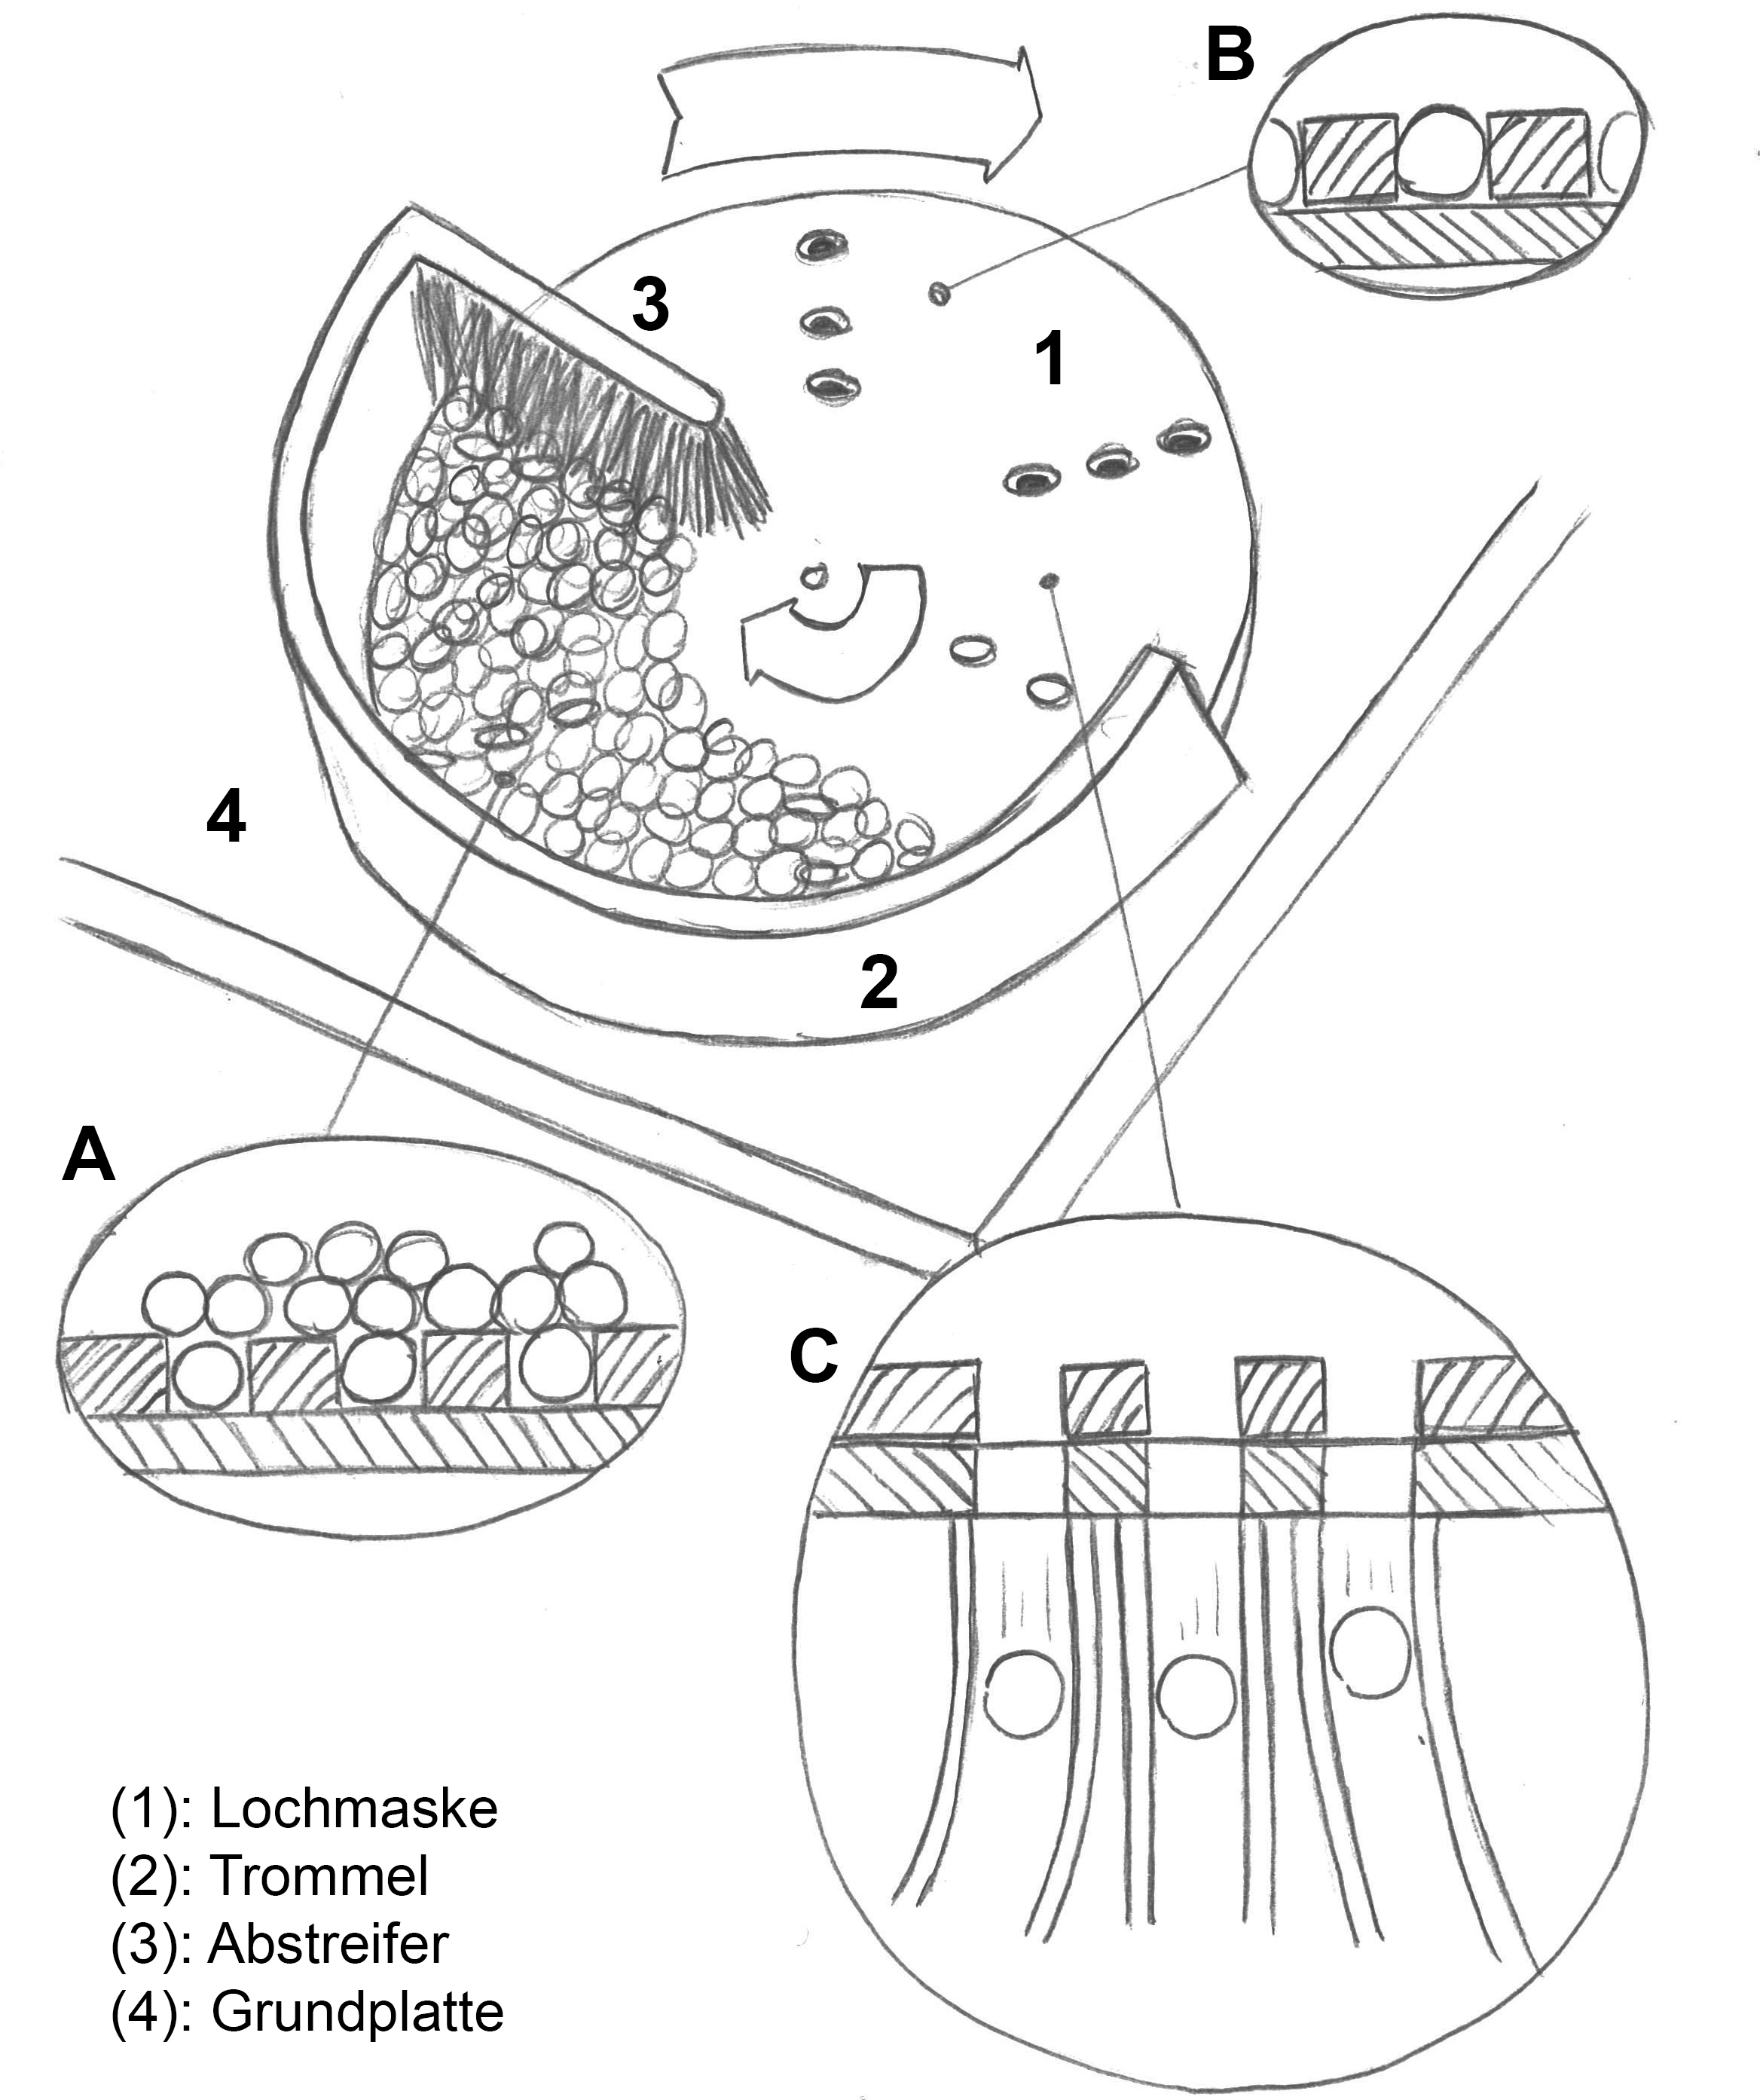
\includegraphics[scale=0.52]{Illustrationen/5-Konzept/schema_vereinzelung.jpg}
	\caption{Vereinzelung durch rotierende Lochmaske}
	\label{fig:schema_vereinzelung}
\end{wrapfigure}
Die Vereinzelung wird im Konzept  Blau durch eine rotierende Lochmaske realisiert. Die NemaCaps werden in einen Behälter gefüllt (Punkt 2 in Abbildung \ref{fig:schema_vereinzelung}). Darin befindet sich eine rotierend-gelagerte Scheibe mit Löchern (Lochmaske, 1). Die Öffnung ist so gestaltet, dass ein NemaCap hineinpasst. Durch die Rotation der Lochmaske fallen nun NemaCaps in die Löcher (Detail A) und werden zu Detail B transportiert. Ein Abstreifer (hier in Form einer Bürste) sorgt dafür, dass überschüssige NemaCaps zurückgehalten werden. In der Grundplatte (4) sind Löcher vorgesehen, welche die NemaCaps in Schläuche fallen lassen (Detail C). Idealerweise wird dieser Aufbau schief gelagert. 
\newline
Dieses Konzept wird von der Firma Kofatec GmbH erfolgreich für die Vereinzelung von Pfefferkörnern eingesetzt. 

\subsubsection{Setzen der NemaCaps durch Ausheben eines Setzloches}
Der Setzprozess von Konzept blau besteht aus zwei Phasen.

\begin{itemize}
	\item \textbf{Ausheben des Setzloches:} In diesem Arbeitsschritt wird die Setzeinheit, durch eine entsprechend translatorisch gelagerte Führung, vertikal in Richtung Topf bewegt. Durch die auf der Setzeinheit zu unterst montierten Stechdornen (Abb. \ref{fig:blau_setzeinheit}, 4) werden drei Löcher in die Topferde gestochen. Beim anschliessenden Anheben der Setzeinheit behalten die Löcher, aufgrund der feuchten Beschaffenheit der Topferde, ihre Kegelförmige Kontur.
\newpage	
	\item \textbf{Platzieren der Nemacaps:} Noch während sich die Setzeinheit zurück in ihre Ruheposition (Abb. \ref{fig:blau_setzeinheit}, rechts) bewegt, werden die Nemacaps durch die Vereinzelung ausgelöst. Von der Vereinzelung ausgelöst, fallen diese mit Hilfe der Schwerkraft in Richtung Setzlöcher. Die Stechdornen dienen in dieser Zeichnung zusätzlich als Führung der Fallbahn, indem sie innen Hohl sind.
\end{itemize}

\begin{figure}[H]
	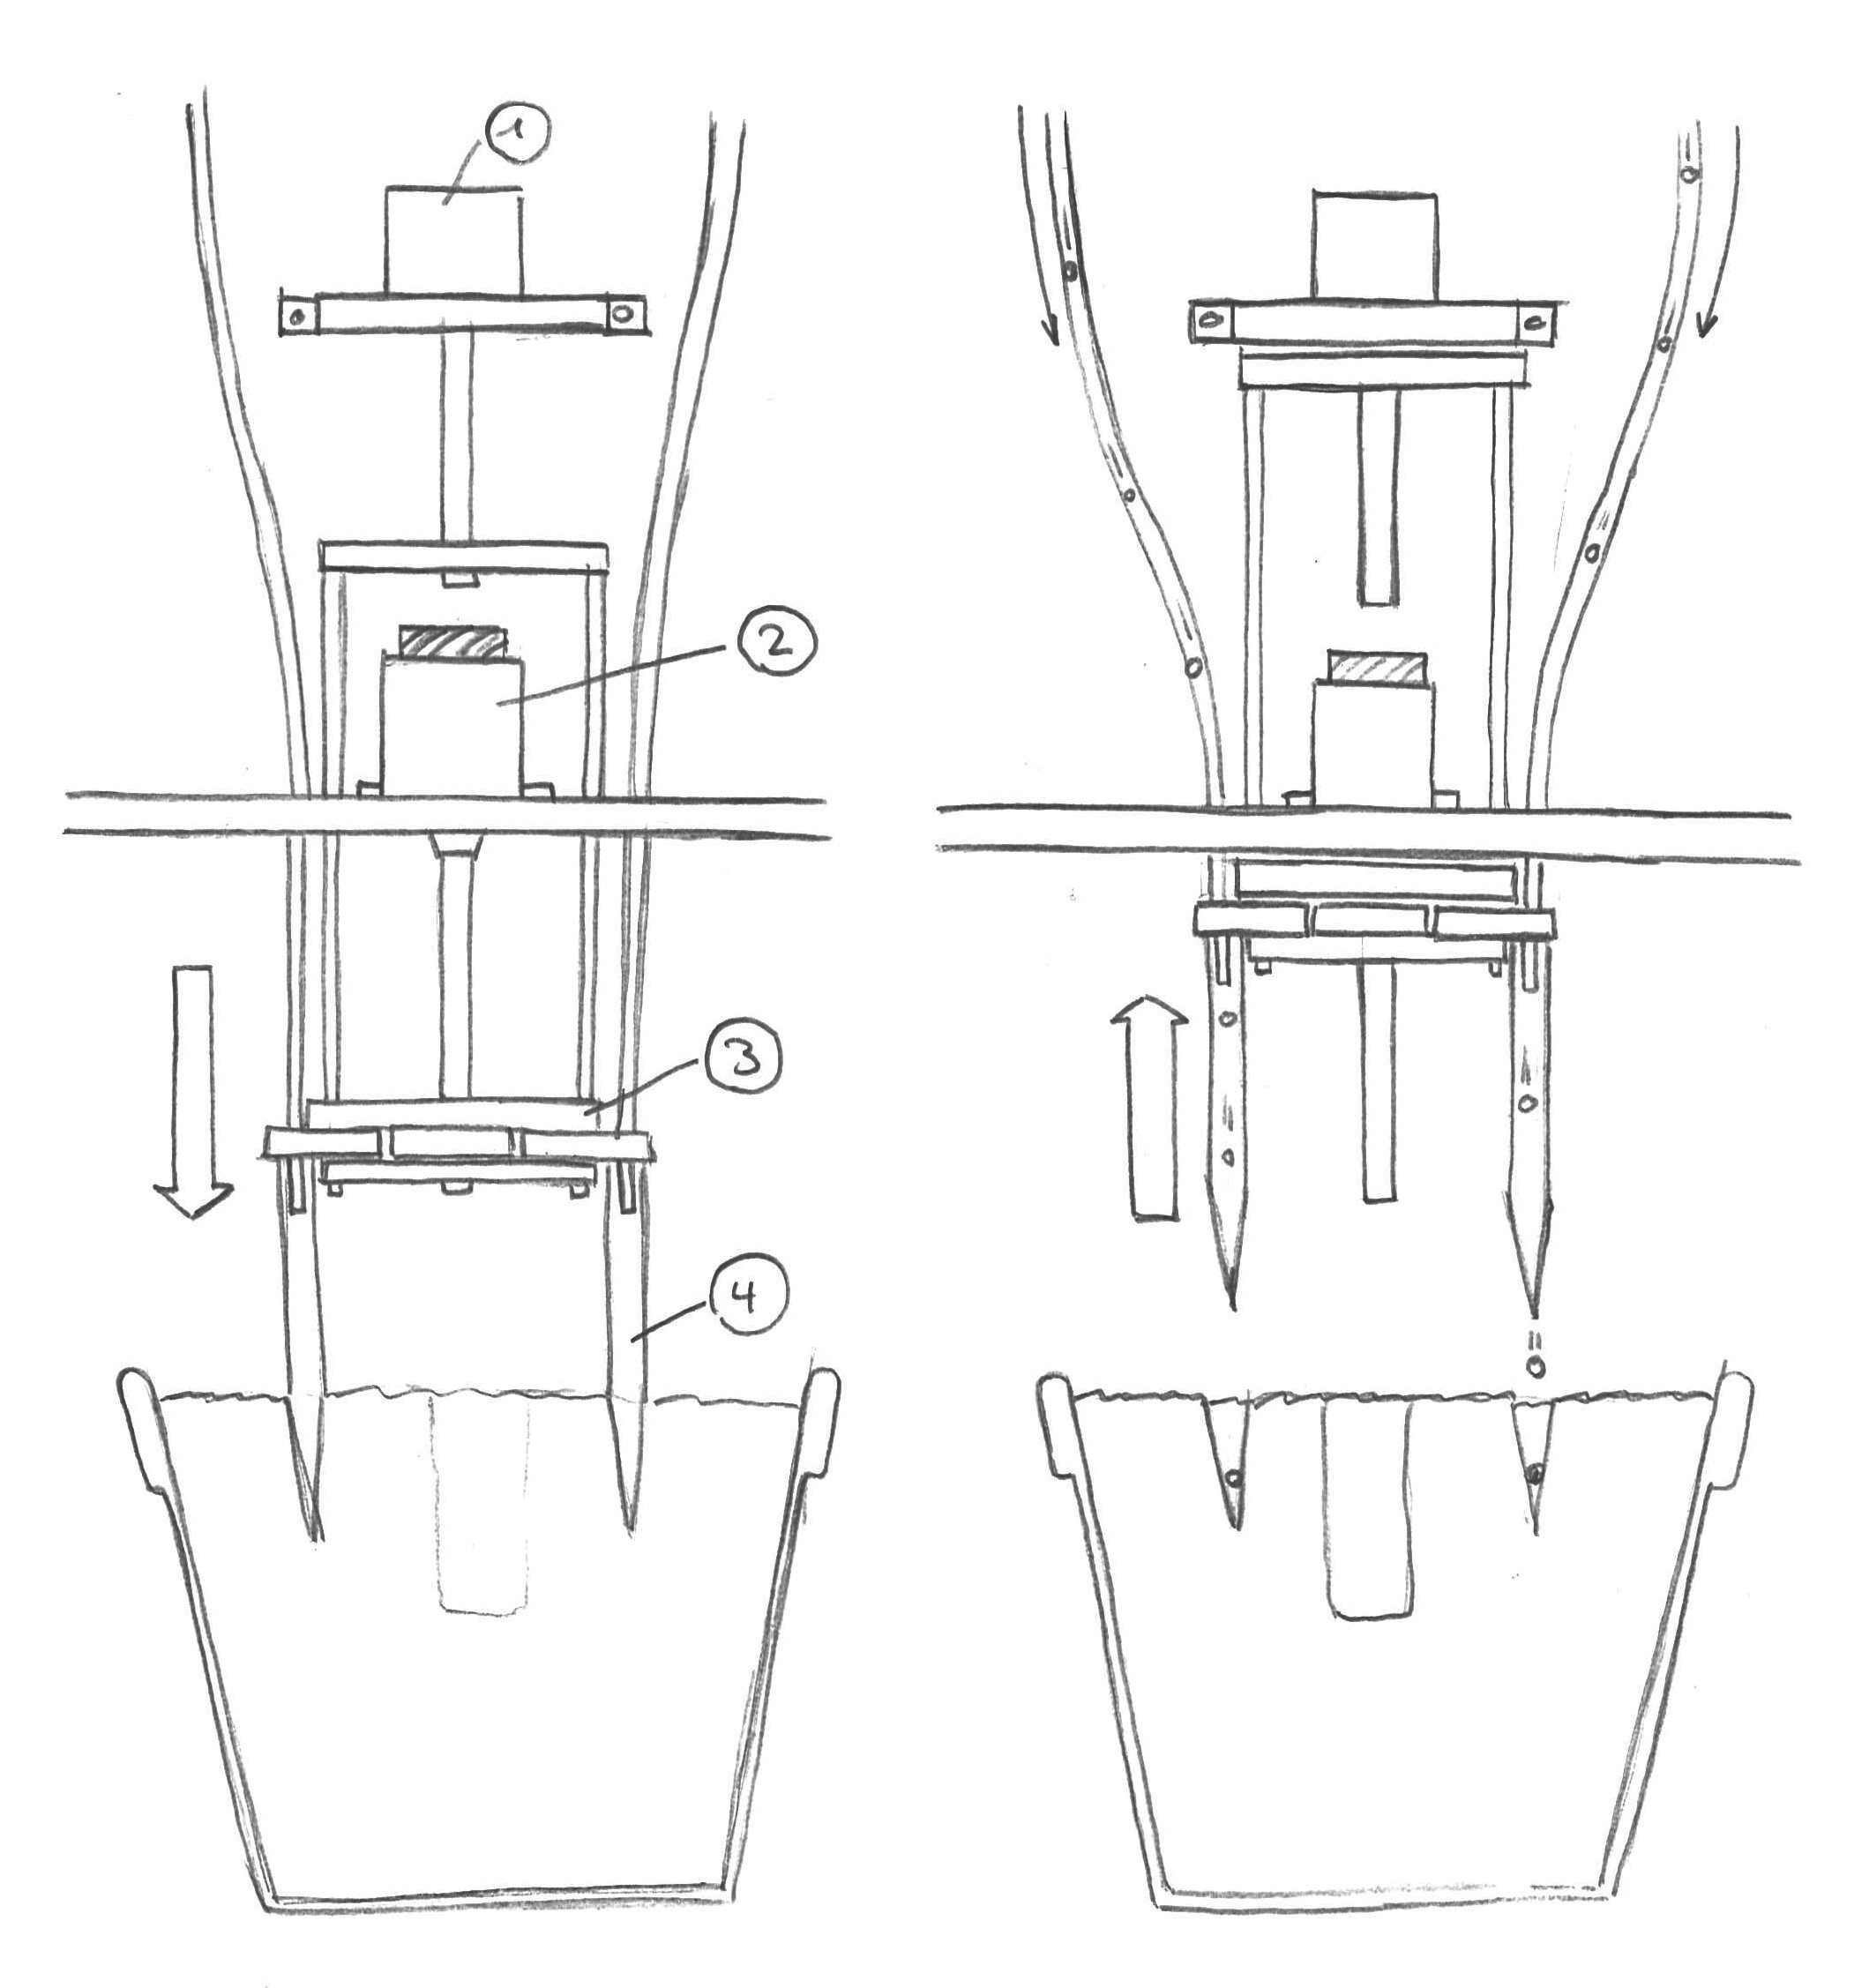
\includegraphics[draft=false,width=0.9\textwidth]{Illustrationen/5-Konzept/blau_Setzeinheit_ohneLegende.jpg}
	\caption{Teilfunktionsmuster zum Setzen der NemaCaps}
	\label{fig:blau_setzeinheit}
\end{figure}

Um die translatorische Bewegung der Setzeinheit zu realisieren, wird ein linear Antrieb benötigt. Dieser ist in der Funktionsskizze beispielhaft als Spindelantrieb ausgeführt (Abb. \ref{fig:blau_setzeinheit}, 1). Die portale Bauweise von Konzept Blau ermöglicht eine Positionierung der Verstellmechanik (Abb. \ref{fig:blau_setzeinheit}, 3) direkt oberhalb der Stechdornen. Der Antrieb der Verstellmechanik wird durch einen stationären Motor realisiert (Abb. \ref{fig:blau_setzeinheit}, 2), welcher eine Keilwelle antreibt. Die bewegte Verstellmechanik wird über die entsprechende Keilnabe angetrieben.

\subsubsection{Setzmechanismus konfigurieren}
Durch die Verstellmechanik Abb. \ref{fig:blau_verstellmech} können die Stechdornen der Setzeinheit auf verschiedene Stechradien eingestellt werden. Die Verstellbarkeit kann dabei dabei durch die Verwendung verschiedener Mechanismen realisiert werden. 
\begin{figure}[H]
	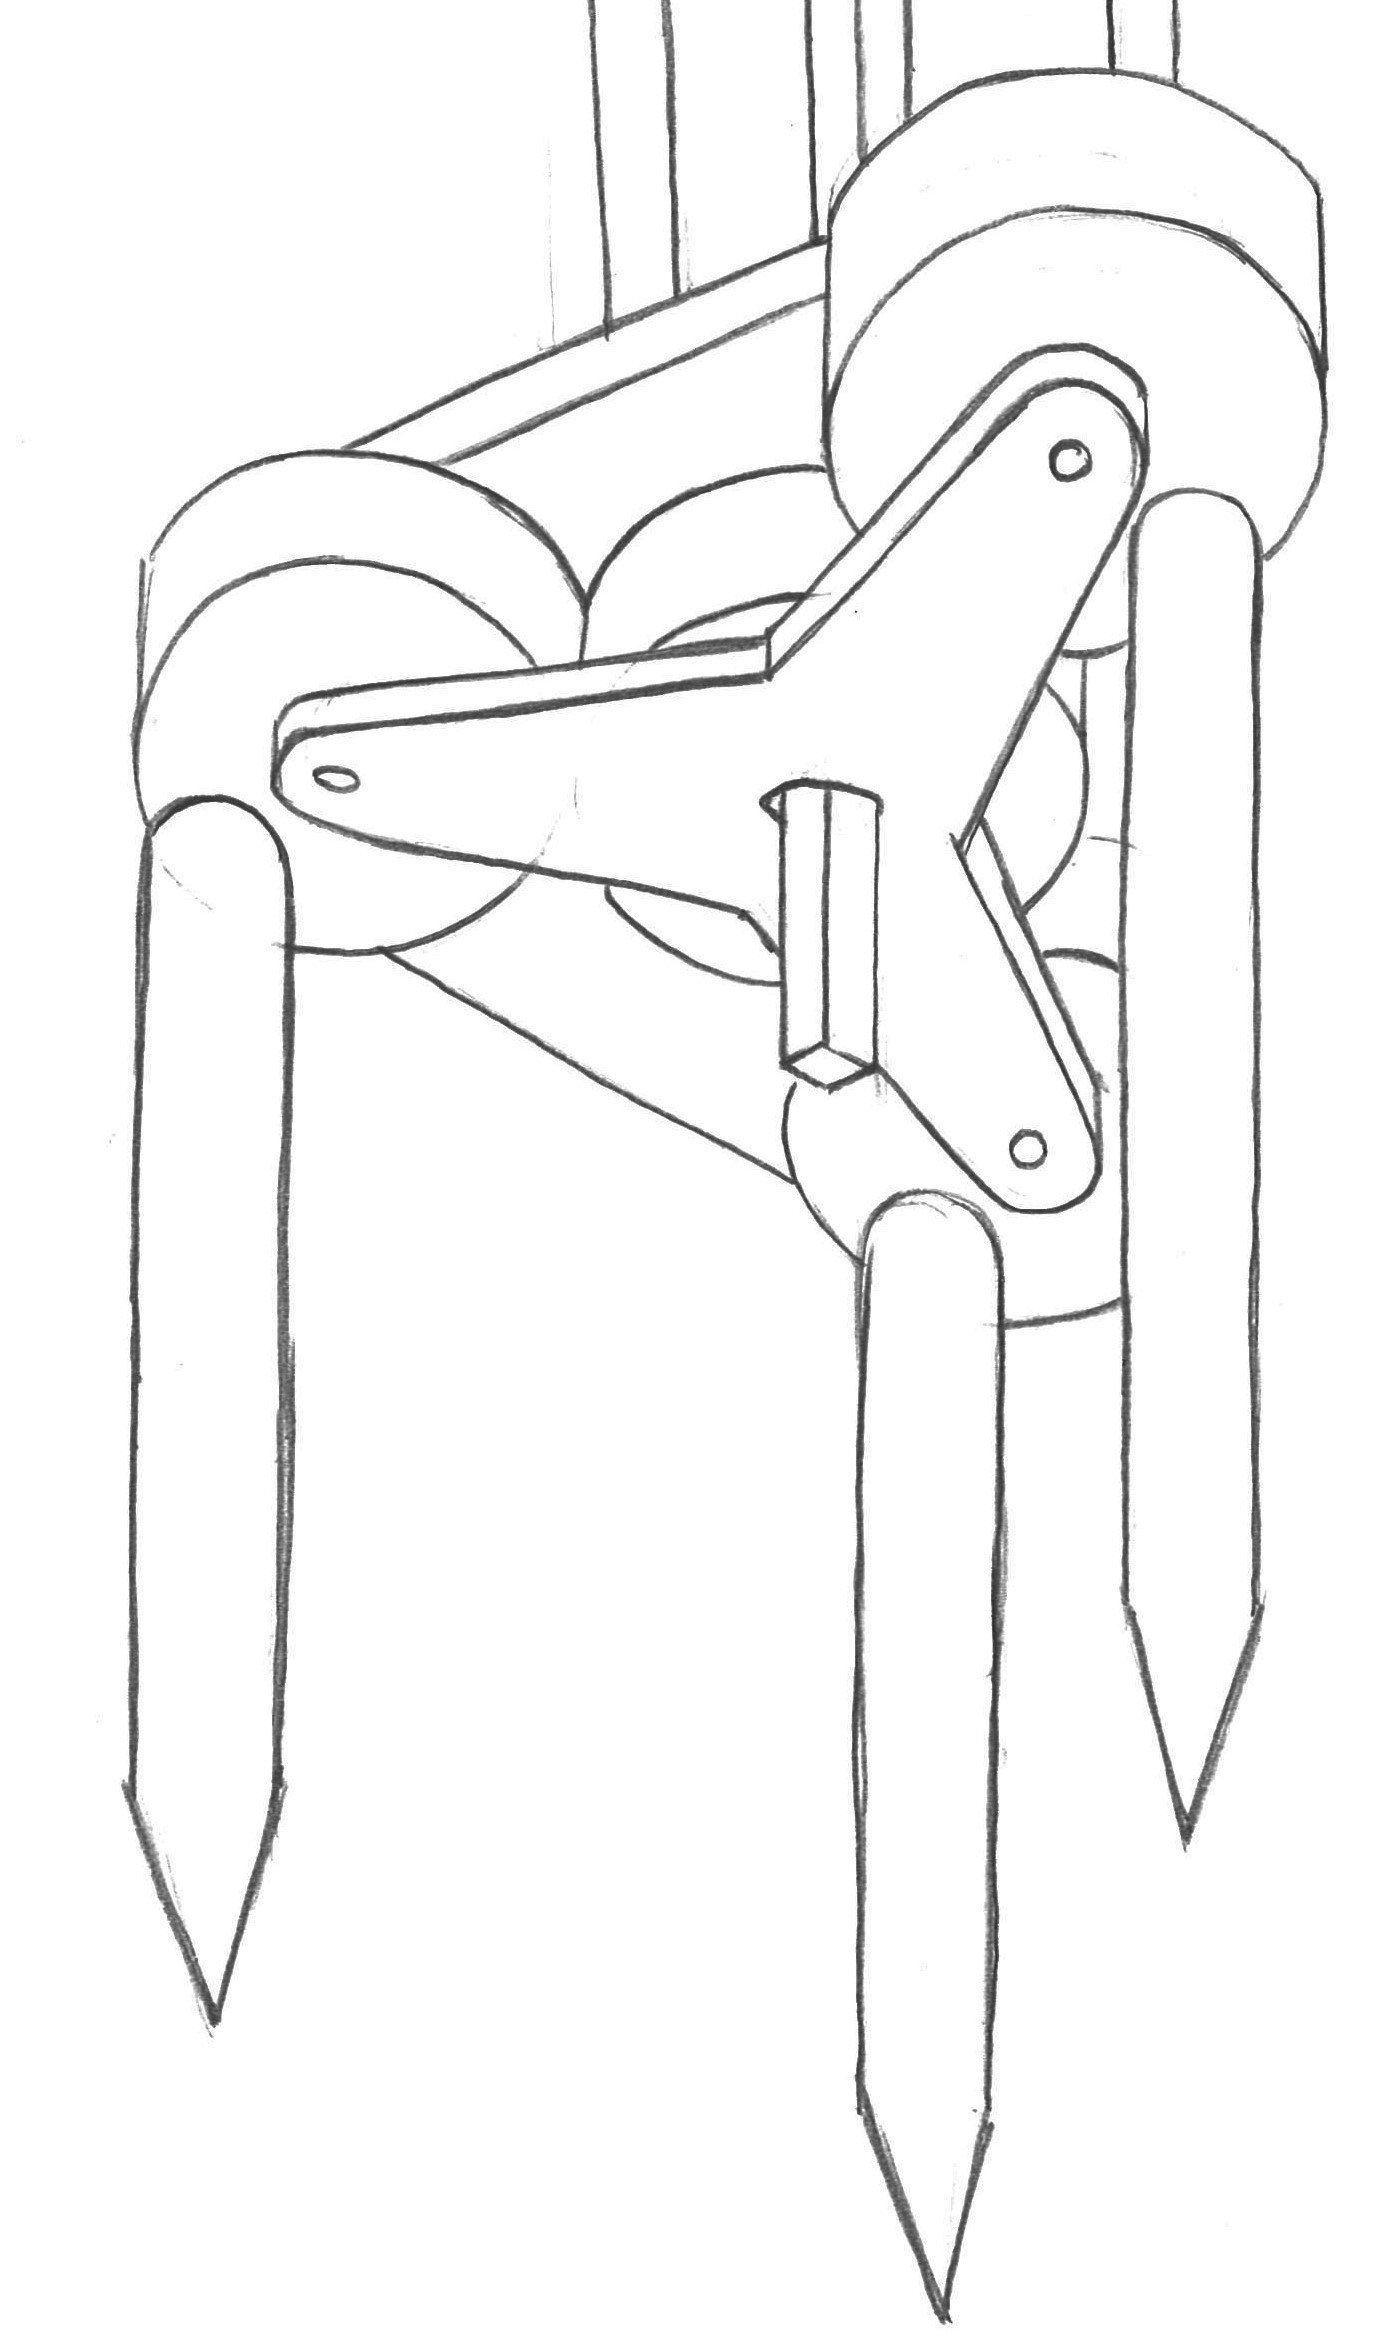
\includegraphics[scale=0.55]{Illustrationen/5-Konzept/blau_Verstellmechanismus.jpg}
	\caption{Teilfunktionsmuster zum konfigurieren des Setzradius}
	\label{fig:blau_verstellmech}
\end{figure}

In folgender Auflistung sind ein paar Ideen für das Design der Verstellmechanik genannt:

\begin{itemize}
	\item Es könnte eine Art Planetengetriebe, ohne dessen Hohlrad verwendet werden. Hierbei würde die Drehbewegung der Keilnabe mittels eines Übersetzungsverhältnis an die Stechdornen weitergegeben. Diese müssten dabei exzentrisch auf ihrem jeweiligen Planetenrad angeordnet sein.
	\item Die Stechdornen könnten durch entlangführen an einer spiralförmigen Kulisse eine radiale Bewegung beschreiben.
	\item Durch eine dreifache Nockenwelle könnten die federgelagerten Stechdornen radial verstellt werden. Dabei würden durch drehen der Nockenwelle alle Stechdornen nach aussen gedrückt. Eine entsprechend positionierte Feder würde die Stechdorne, bei einer Drehung der Nochenwelle auf den kleinsten Radius, wiederum zurück drücken.
\end{itemize}

